\documentclass[twoside]{article}
\usepackage{graphicx}
\usepackage{amsfonts}
\usepackage{amsmath}

\usepackage[top=4cm, bottom=4cm, left=4cm, right=4cm]{geometry}
%\usepackage[cm]{fullpage}

\usepackage{fancyhdr}


\pagestyle{fancy}
\fancyhead{}
\fancyfoot{}

\fancyhead[RO, LE]{\thepage}
\fancyhead[CE]{HENRY A. KIERSTEAD}
\fancyhead[CO]{RECURSIVE ORDERED SETS}
\renewcommand{\headrulewidth}{0pt}
\renewcommand{\footrulewidth}{0pt}

\begin{document}

\begin{flushleft}
Contemporary Mathematics\\
Volume 57, 1986
\end{flushleft}







\begin{center}
RECURSIVE ORDERED SETS\\
Henry A. Kierstead
%\maketitle
\end{center}
§ 1 Introduction\\
\indent
Many mathematicians working in finite combinatorics are highly suspicious of infinite sets and structures.   This suspicion does not extend to all infinite structures.   
The set of natural numbers with the usual order is considered quite acceptable and, on the whole, so is the set of real numbers with its usual order.   
The problems arise when some unusual structure is placed on these sets as in well ordering the real numbers.   
Other examples arise from extending theorems about finite structures to theorems about infinite   structures.    
Once Dilworth's Theorem has been proven for finite ordered sets it is routine to extend it to infinite ordered sets of finite width via the Compactness Theorem.   
However the resulting structure may be quite unusual.   
The proof only shows the existence of a chain cover; it does not produce the chain cover.   
This is the source of the uneasiness in both cases:    The structures whose existence is asserted have not been shown to be available for inspection.\\
\indent
Rather than ignoring these existence results one should go one step further and ask whether there is a satisfactory structure available for inspection. 
This leads to further questions. What does it mean to be available for inspection? 
How would you show that there was no satisfactory structure available for inspection? 
For countable structures these concerns can be made precise and can often be resolved using the theory of recursive (i.e. computable) functions.   
The resulting combinatorial theory is the subject of this article, which in particular will'concentrate on antichain covers, chain covers, and realizers of recursive ordered sets.\\
\indent
Let us agree that a structure is available for inspection if it is recursive, where, roughly speaking, a relational structure   P   is recursive if it is recursive, where, roughly speaking, a relational structure P is recursive if\\
\newline
---------------\\
1980 Mathematics Subject Classification. Primary 03D45. supported by ONR grant N00014-85K-0494
\newline

\begin{flushright}
© 1986 American Mathematical Society 0271-4132/86 $1.00 + $.25 per page
\end{flushright}

\newpage

there is a finite algorithm that will provide yes-no answers to questions of the form:  "Is    x    in the domain of    P?" and "Does $\bar{x}$    hold for the relation R?"  We shall see that the uneasiness resulting from the use of the Compactness Theorem is well founded,  for there exist recursive ordered sets (necessarily infinite) with finite width   w   that   cannot be covered by w recursive chains.    
Two reasonable responses to this negative result are the traditional recursion theoretic response of analyzing the "degree of non-computability" of such a cover and the more recent combinatorial response, which we shall pursue, of searching for a recursive chain cover that uses some finite number of additional chains. 
Thus we are asking whether there exists a function b such that every ordered set with fini te width w, which is available for inspection, has a chain cover consisting of b(n) chains, which is available for inspection. 
From a finite point of view this approach leads to a very satisfying theory. 
There can be no doubt that the structures under consideration really exist. 
They are essentially finite since they can be stored using only finitely much space by storing the finite algorithms that describe them.    
They are amenable to the type of explicit construction often used on finite structures.    
The results we prove are quite interrelated. Recursive antichain covers and recursive realizers are used to construct recursive chain covers while recursive chain covers are used to construct recursive realizers.
The proofs rely most heavily on algorithmic techniques and the theory of finite ordered sets.    
Indeed, essentially all the recursion theory needed can be reduced to two lemmas. 
The goal of this article is to present a collection of results, proofs, and problems on recursive ordered sets in a unified setting, which is accessible to discrete mathematicians with little or no background in recursion theory.\\
\newline
For the most part our notation is standard; a few special conventions are mentioned here. The set of natural numbers is represented by n. 
Incomparability in ordered sets is denoted by $\Vert$. The restriction of a structure (a,$\bar{R}$) to the substructure generated by B $\subset$ A is denoted by (a,$\bar{R}$)$\vert$B.\\


§2   K - L   Expansion Theorems\\


In this section we use the language of general relational structures to define the notion of an expansion theorem.   Next we review the basics of elementary recursion theory and present the notion of a recursive expansion theorem.    Finally we introduce expansion games and prove two lemmas which reduce the proofs of recursive expansion theorems to finding winning strategies in expansion games.   These games are interesting in their own right and are related to on line algorithms.

\newpage

A (relational) i \underline{structure} is a system   A = (A, $\bar{R}$)   where   $\bar{R}$   is a sequence of relations on the domain   A.   
To avoid certain technical difficulties we will only consider structures with finitely many relations.    
Structures will be denoted with bold face letters;  the same letter in standard form will denote the domain of the structure.   
Two structures (A,$\bar{R}$)   and   (B,$\bar{S}$) are similar    provided that   $\bar{R}$   and   $\bar{S}$ have    the same length and corresponding entries in   $\bar{R}$   and    $\bar{S}$   have the same rank.    The structure
$(A,R_1,...,R_m...,R_n)$    is an \underline{expansion} of  the structure    $(A,R_1,...,R_m)$.    
Let K be a class of similar structures and let   L   be another class of similar structures.   
A   K - L   \underline{expansion} \underline{theorem} is an assertion of the form: Every structure in   K   has an expansion in   L.    Dilworth's Theorem is an example of a   K - L   expansion theorem. Matching theorems, coloring theorems, and dimension theorems for ordered sets also fall into this category.

There are many equivalent ways to define the concept of a partial recursive or computable function.    
For our purposes it will be enough to say that a \underline{partial} \underline{recursive} \underline{function}  $\Phi$    is a function that can be computed by an algorithm of finite length - if   x   is in the domain of $\Phi$ then the algorithm eventually produces the output $\Phi(x)$ when started on the input   x; if   x is not in the domain of     the algorithm produces no output when started on the input   x.   
A \underline{recursive} \underline{set} is a set whose characteristic function is recursive. 
Notice that every finite set is recursive. A precise definition of these concepts can be found in Machtey and Young [1978].   
The domain of a partial recursive function may not be recursive; if it is we will say that the function is recursive.   
This is a slight variance from the normal definition. 
A structure   A   = (A,$\bar{R}$)    is \underline{recursive} if there is a recursive function  such that both $\Phi(0,x) = 1$   iff   x $\in$ A   and $\Phi(R, \bar{x}) = 1$   iff   $x\in R$, whenever R is in $\bar{R}$. We say that $\Phi$   defines   A.   
If   A   is a recursive structure the domain of   A     and each of its relations are recursive sets.   
To test whether x   is in   A, first check whether   (0,x)   is in the recursive set   dom($\Phi$) and if it is check to see whether   $\Phi(0,x) = 1$.
It is also easy to see that if each of the relations of   A   is recursive and the domain of   A   is recursive then   A   is recursive.   
Thus the domain and each of the relations of a recursive structure are completely described by a single algorithm of finite length. 
A \underline{recursive} K-L \underline{expansion} \underline{theorem} is an assertion of the following form: Every recursive structure in K has can be expanded to a recursive structure in L.\\ 
\indent It is possible to enumerate the countably many possible algorithms. 
Let $\Phi_e$   be the partial recursive function computed by the eth algorithm in such a list.   
The execution of      algorithm on a particular input occurs in a step by step manner.    
If the execution of the   eth   algorithm   on   x   halts after at most   n   steps and outputs   y   we say that   $\Phi_e^n(x)$   is defined and equals y;
\newpage


\noindent otherwise we say that  $\Phi_e^n(x)$    is undefined.   With special care (Kleene [ 1936], Turing [1936]) we can arrange the list so that the predicate   T = \{(e,x,n): $Phi_e^n(x)$   is defined\} is recursive.    
Thus in writing algorithms we can use statements of the form: if $\Phi_e^n(x) = y$ then ...  .    In general we can not use statements of the form:  if    $\Phi_e(x) = y$ then. . . , since there is no algorithm that will decide for arbitrary   e   whether the   eth   algorithm eventually produces output when started on the input   x.    
For further details the reader should consult Machtey and Young [1978].\\


The   K - L   \underline{expansion} \underline{game} is an infinite game played by two players, the K-player and the   L-player,  in the following fashion:    The play alternates between the two players with the   K-player moving first. 
At the start of the i+1st round of play    the K-player will be confronted with a finite structure $B = (B, R_1,...,R_m,...,R_n)$    in   L, which is the expansion of a K-structure $B = (B,R_1,..., R_m)$.    
The   K-player must define new relations $R_1^{+},...,R_m^+$     on $B^+ = B \cup \{i\}$   such that   $B^+ = (B^+, R_1^+,...,R_m^+)$ is in   K   and   B   is a substructure of $B^+$, i.e., $x\in R$. iff $x\in R_i^+$ for all x in B and $1 \leq i \leq m$. 
The L-player responds by defining new relations   $R_{m+1}^+,...,R_n^+$ on   $\bar{B}^+$   such that   $\bar{B}^+ = (B^+,R_1^+,...,R_m^+,...,R_n^+)$    is   in   L   and   B is a substructure of   $\bar{B}^+$.   
The K-player \underline{wins} a   K - L   expansion game if after finitely many rounds of play the L-player has no legal response;  the L-player wins if the game continues for infinitely many rounds or in the unlikely event that the   K-player cannot play legally.\\
\indent A \underline{strategy} \underline{for} \underline{the}   K-\underline{player} is a function   S which assigns to each finite L-structure $\bar{B}$ with $\bar{B} = \{0,1,...,i-l\}$ a structure   $S(\bar{B}) = \bar{B}^+$. 
The strategy S is a \underline{winning} \underline{strategy} if regardless of how the   L-player responds the K-player can eventually win the   K - L   expansion game by continuing to play $S(\bar{B})$ when confronted with   $\bar{b}$.
Similarly a \underline{strategy} for the   L-\underline{player}   is a function   S   that assigns to each pair of structures  $\bar{B}$   in   L and   $B^+$   in K such that   $B^+ = B \cup \{i\}$   a structure   $S(\bar{B},B^+) = \bar{B}^+$.   The strategy   S   is a winning strategy if regardless of how the   K-player moves the L-player wins by always responding with   $S(\bar{B},B^+)$   when confronted with   $\bar{B}$   and $B^+$.\\
\indent It is a consequence of K\"{o}nig's Lemma   that if the   K-player has a
winning strategy for the   K - L   expansion game then there is a fixed   n such that regardless of how the   L-player responds the   K-player can win in at most n   rounds:   Consider the tree, whose nodes are the   L-structures that can start some round of a   K - L   expansion game in which the K-player follows his winning strategy, and whose nodes are ordered by the substructure relation.
This tree is finitely branching.    If the   L-player could force arbitrarily long games, then the tree would be infinite, and by K\"{o}nig's Lemma would contain an infinite branch, which would correspond to a winning game for the
\newpage
\noindent L-player playing against the   K-player's winning strategy.    
Thus if the K-player has a winning strategy that strategy can be chosen to be finite and thus recursive.    
On the other hand, it is conceivable that the L-player has a winning strategy, which is so complex that it cannot be described by an algorithm.


The reminder of this section is devoted to reducing the recursive
theorems to follow to game theoretic results.    In order to state the crucial
lemmas we need to define several operations on structures. The \underline{union} \underline{of} underline{a}
\underline{chain} of similar substructures $(A_0,\bar{R}_0) \subset (A_1,\bar{R}_1) \subset ...$ denoted by
$(A,\bar{R}) =  \bigcup_{i\in N}(A_i,\bar{R}_i)$,  is defined by   $A = \bigcup_{i\in N} A_i$ . and   $\bar{x} \subset R$ iff $\bar{x} \in R_i$, for
some   $i \in N$, where   R   and   $R_i$    are corresponding relations in   $\bar{R}$   and   $\bar{R}^+$.
Let   $A = (A,\bar{R})$   be a structure and   f   be   a bijection from A to   B. The
\newcommand{\meph}{\mathbf}
\underline{isomorphic} \underline{image} of A under f is the structure   $\meph{B} = (B,\bar{S})$ defined by
$(x_j,...,x_r)\in R$ iff $(f(x_i),...,f(x_r)) \in S$, where   R   and   S   are corresponding
relations in   $\bar{R}$   and  $\bar{S}$. Let   $\meph{A} = (A,\bar{R})$   be a structure and suppose that for
each   $a\in A, \meph{B_a}   = (B, S)$ is a structure similar to $\meph{A}$ such that $B_a \bigcap B_{a'} = 0$ if $a \neq a'$.
The \underline{sum} \underline{over}   $\meph{A}$   of the $\meph{B_a}$, denoted by   $(B,\bar{S}) =  \sum_{\meph{a}\in \meph{A}} B_a$   is defined by
and $\aleph = (x_1,..., x_n)\in S$ iff either $\bar{x} \subset B_a$   and $\bar{x} \in S_a$, for some $a \in A$
or $\bar{x} \not \subset B_a$   for any $a \in A, x_t \in B_{a(i)}$, and   $(a(l),. .. ,a(n)) \in R$,   where   $S, S_a$, and
R   are corresponding relations in $\bar{S}, \bar{S_a}$, and $\bar{R}$.
Let K be a   class	of similar structures and let A be a structure similar to the structures in	K. 
We say that   K   is closed under the formation of, respectively, substructures,
unions of chains, isomorphic images, and sums over   A, provided   B	is in K
whenever   B   is, respectively, a substructure of a structure in   K,	a union of
a chain of substructures in   K, the isomorphic image of a structure	in   K, or
a sum over A   of structures in K.\\
\newline
\underline{Lemma} 1.   Suppose   K   is a class of similar structures closed under	the
formation of substructures and isomorphic images and   L   is a class	of similar
structures closed under the formation of unions of chains.    If the	L-player
has a recursive winning strategy for the   K - L   expansion game,  then every
recursive structure in   K   can be expanded to a recursive structure	in L.\\
\newline
\underline{Proof}.     Let $B = (B,R)$ be a recursive structure in   K.   The recursive expansion   $\bar{B}$ of $B$ is obtained from a run of the K-L expansion game. 
For notational simplicity, using that K is closed under the formation of isomorphic images, assume that   $B = n$, and suppose that at each round   s   the K-player plays   $\meph{B^s} = \meph{B}(0,1,...,s-1)$   while the   L-player uses his recursive winning strategy to respond with  $\meph{\bar{B}^s}$.   
Since   K   is closed under the formation of substructures each play by the   K-player is legal and the game continues until -each point of   B   has been enumerated.   
The resulting structure   $\bar{B}$   is clearly
\newpage
%
% STRONA 6
%
an expansion of $\meph{B}$. 
Since $\meph{\bar{B}}$ is the union of the chain of structures $\meph{\bar{B}^s}$ played by the L-player and L is closed under unions of chains, $\meph{\bar{B}}$ is in L. 
The domain B is recursive since $\meph{B}$ is. 
Since $\meph{B}$ and S are recursive one can effectively calculate the posi tion of the game after any finite number of rounds. Thus we can effectively determine whether or not any of the relations of $\meph{\bar{B}}$ hold for a sequence $\bar{x}$ by allowing the game to run until each point in $\bar{x}$   has appeared.    
Hence   $\meph{\bar{B}}$  is recursive.$\Box$\\
\newline
\underline{Lemma} 2.    Suppose that A   is an infinite recursive structure, K   is a class of structures similar to   A   such that   K   is closed under the formation of isomorphic images and sums over A, and   L   is a class of similar structures closed under the formation of isomorphic images and substructures.
If the K-player has a winning strategy in the   K - L   expansion game then there is a recursive structure in   K   that cannot be expanded to a recursive structure in L.\\
\newline
\underline{Proof}.    Let   S   be a finite winning strategy for the   K-player in the   K - L expansion game and   p   be a recursive bijection from N   to N x N. Without loss of generality assume that   A =   N.    
Like a chess master, we shall simultaneously play infinitely many K-L expansion games against every possible recursive strategy for the L-player, using the K-players winning strategy. 
The order in which we visit the various boards will be governed by the function p. The result will be a recursive structure B in R which cannot be expanded to a recursive structure in L.


\underline{Algorithm} \underline{for} \underline{B}:   The algorithm proceeds in stages.   At stage s we construct $\meph{B^s}$.    After   $\omega$   stages we let   $\meph{B} = \bigcup_{s\in N} \meph{B^s}$.\\
\underline{Stage} 0.    Set $f_e^0 = \emptyset = \meph{B_e}^0$    for all $e\in N$.
\underline{Stage} s+1.   Suppose p(s) = (e,i). If $d\neq e$  set $f_d^{s+1} = f_d^s$ and $\meph{B}_d^{s+1}=\meph{B}_d^s$.   If $\Phi_e^s$
defines an expansion of $\meph{B}_e^s$  to a structure  $\meph{\bar{B}}_e^s$whose preimage $\meph{\bar{C}}_e^s$ under $f_e^s$   is in
L set $f_e^{s+1} = f_e^s \cup \{(|\meph{B}_e^s|,s)\}$ and $\meph{B}_e^{s+1} = f_e^{s+1}[S(\meph{\bar{C}}_e^s)]$; otherwise set $f_e^{s+1} = f_e^s$
and $\meph{B}_e^{s+1} = B_e^s$.    Let   $\meph{B}_e^{s+1} = \sum_{e\in N} \meph{B}^{s+1}$.


The predicate  "$\Phi_e^s$  defines an expansion of	$\meph{B}_e^s$ whose preimage under $\bar{C}_e^s$ under $f_e^s$ is in   L" is easily seen to be recursive since $\meph{B}_e^s$ is finite, "$\Phi_e^s(x)$ is defined" is a recursive predicate, and if $\bar{C}_e^s$   is in   L then $\bar{C}_e^s$   is one of the only finitely many legal positions which can be reached during a run of the K - L expansion game with the K-player using his finite winning strategy S. Using also that  A is recursive we see that we can effectively construct each $\meph{B}^s$.   Thus as in the proof of Lemma 1, $\meph{B} = \cup_{s\in N} \meph{B}^s$.   is recursive.
\newpage
%
% STRONA SIÓDMA
%


To see that   B is a K-structure note that $B =  \bigcup_{s\in N} \sum_{e\in A} \meph{B}_e^s = \sum_{e\in A} \bigcup \sum_{s\in N} \meph{B}_e^s$ 
and that for each   e    there exists a stage    t such that $\bigcup_{s\in N} \meph{B}_e^s = \meph{B}_e^t$.    Set i $\meph{B}_e = \meph{B}_e^t$.    Since   K is closed under the construction of images of isomorphisms and
sums over   A, each  $\meph{B}_e$ is in   K and thus $\meph{B}$ is in K.\\
\indent Finally suppose that $\meph{\bar{B}}$ were a recursive expansion of B. Then $\meph{\bar{B}}$ would be
defined by some partial recursive function $\Phi_e$ which would also define an
expansion $\meph{\bar{B}}_e$   of $\meph{B}_e$. Since L is closed under the formation of substructures and images of isomorphisms, $\meph{\bar{B}}_e$ and its preimage $\meph{\bar{C}}_e$     would be in L, which would
contradict   $\bigcup_{s\in N} \meph{B}_e^s = \meph{B}_e$. $\Box$\\



\noindent\S 3   Recursive Antichain Covers\\
\newline
\indent We begin our study of recursive ordered sets with recursive antichain covers, since as one might expect from the finite case,  the results are relatively easy to prove.   
Every ordered set of finite height (the number of points in a maximum chain) h   can be covered by   h   antichains. 
Schmerl proved the following recursive version of this result.\\
\newline
\underline{Theorem} 1.(Schmerl [1979])   Every recursive ordered set of finite height h can be covered by $\binom{h+1}{2}$  recursive antichains; moreover for all positive integers   h there are recursive ordered sets of height   h   that cannot be covered by less than $\binom{h+1}{2}$ recursive antichains.\\
\newline
\underline{Proof}. Let K be the class of ordered sets P = (P,R) of height at most h and let L be the class of all structures of the form $\bar{P} = (P,R,A_1,...,A_n)$ where (P,R) is in K, $(A_1,...,A_n)$ is an antichain cover of P, and $n = \binom{h+1}{2}$. Note that K and L satisfy the hypothesis of Lemma 1. 
To prove the first part of the theorem we provide the L-player with a recursive winning strategy for the K-L expansion game. Relabel the antichains $A_1,...,A_n$ as $..,A_d,_u...$ where $0 \leq d+u \leq h-1$.   
When confronted with a new point i in the
finite ordered set $P^+$ the L-player should put i in the antichain $A_{d,u}^+$   , where d  is the length of the longest chain in P   strictly below i and u is the
length of the longest chain in $P^+$ strictly above i.   This is a recursive
winning strategy: We have (informally) provided the finite algorithm for
computing the next move from any position, so the strategy is recursive. To
see that it wins, it suffices to show that each $A_{d,u}^+$  is still an antichain.
Suppose $i$ is comparable to $x$ and $x \in A_{d,u}$, say $i < x$. Then there is a chain of $u + 1$ elements strictly above $x$. Thus $i \not \in A_{d,u}^+$.\\
\indent The second part of the theorem is contained in Theorem 2, a stronger (and later) result of Szemer\'{e}di, which will also be used in the proof of Theorem 4.$\Box$

\newpage
%
% STRONA ÓSMA
%


Before presenting Theorem 2, we remark that some care was necessary in designing the winning strategy for the   L-player.   Consider the \underline{greedy} \underline{strategy}:    Put    i    in the antichain  $A_j^+$   of least index such that   $A_j \cup  \{i\}$ is    still an antichain.    
This is not a winning strategy for the   L-player even if we allow him extra antichains.    
To see this, we show that for each positive n    there is a sequence of plays $S_n^+  (S_n^-)$   for the   K-player ending with a
structure $P_n^+  (P_n^-)$   of height   2   such that the last element $x_n$    is maximal
(minimal) and if the   L-player uses the greedy strategy then $x_n$   is put in $A_n$.   The argument is by induction on   n.    Figure 1 illustrates the inductive step.


A collection of linear orders $L = (L_1,..., L_n)$    is a realizer of an ordered set   $P = (P, R)$   provided   $x<y$ in $R$   iff for all $i$, $x<y$ in $L_i$.   $L$   is a recursive   realizer if the structure  $(P,R,C)$ is recursive.    The (recursive) dimension of   $P$   is the least number of linear extensions in a (recursive) realizer of   $P$.\\
\newline
\underline{Theorem} 2.    (Szemer\'{e}di [1982])     For every positive integer   $h$  there exists a
recursive ordered set with height   $h$   and recursive dimension 2 which cannot
be covered by fewer than $\binom{h+1}{2}$	recursive antichains.\\
\newline
\underline{Proof}.    Let $K_h$	be the class of structures   $P = (P,R,L_1,L_2)$   where   $(P,R)$ is
an ordered set of height at most $h$   and  $(L_1, L_2)$   is a realizer of   $(P,R)$; let
$L_h$   be the class of structures $\bar{P} = (P,R,L_1,L_2,A_1,...,A_n)$   such that
$(P,R,L_1,L_2)$   is in	$K_h$ and   $(A_1,...,A_n)$ is an antichain cover of   $P$, where
$n = \binom{h+1}{2}-1$; and let $A = (A,S,M_1,M_2)$ where $A = N$, $S$ is the empty order, $M_1$
is the natural order on   $N$   and	$M_2$ is the dual of  $M_1$.   Then   $K_h$, $L_h$ and
$A$   satisfy the hypothesis of Lemma 2.   To prove the theorem we provide a winning strategy for the   $K_h$-player in the  $K_h - L_h$   expansion game by recursion on   $h$.    If   $h=1$    the   $L_h$-player cannot respond to any move, so
assume $h = g+1$ and   let  $S_g$     be a winning strategy for the   $K_g$-player in the $K_g - L_g$   expansion game.\\
Note that	$\binom{h+1}{2}	- \binom{g+1}{2} = h$. The   $K_h$-players     strategy consists of two
stages.    The strategy creates a structure   $P = (P,R,L_1,L_2)$, with   $P = P_1 \cup P_2$, where   $P_1$ is the set of points played during the first stage and   $P_2$   is the set of points played during the second stage.   
The goal of the first stage is to arrange that the top   $h$   points, $T$, of   $P_1$   in   $L_1$   are all incomparable in $R$, while tricking the   $L$-player into putting the elements of   $T$   into $h$ distinct antichains.   
The goal of the second stage is to arrange that: $(P2,R,P2)$   has height   $g$; every element of   $P_2$   is under every element
of $T$ in   $R$   and incomparable in   $R$  to every element of   $P_1 - T$;   and the $L_h$-player
\newpage
%
% STRONA DZIEWIĄTA
%
is forced to use $\binom{g+1}{2}$	distinct antichains to cover $P_2$.	Then the   $L$ player
will be forced to use   $h + \binom{h}{2}$	antichains in all and loose.\\
\indent The second stage is easy.    The   $K$-player simply follows the strategy $S_g$
(modified for the points in  $P_2$).    At the same time he relates each new point
$i$	in $P_2$ to the points in $P_1$	by putting $i$ over all the points of $P_1 - T$
and under all the points of   $T$   in   $L_1^+$   and putting   $i$   under all the points
of   $P_1$   in $L_2^+$.
It remains to explain the   $K_h$-players strategy for the first stage.
Suppose the points   $Q_r$   from   $P_1$   have been played so that   $P\lceil Q_r$   has height
at most   $r$, the top   $r$   points   $T_r$   of	$Q_r$ in $L_1$	are all incomparable in
$R$,    and the   $L_h$-player has used exactly   $r$   antichains to cover $Q_r$, each of which contains an element of   $T_r$.    The   $K$-player should add new points $c_1,..., c_i,..., c_j$    to  $P_1$   one at a time, so that   $c_i$    is the   $r + 1$st point in   $L_1^+$   and the top point in   $L_2^+$, until the   $L_h$-player puts  $c_i = c_j$    into a new antichain.    
Note that this will occur at or before a point at which $c_j$ is in a chain of length   $r + 1$   and that such a point will be reached since the set    $(c_1,.., c_j)$    is a chain.   
Continuing in this manner, after replacing $r$   by   $r+1$,   $Q_r$   by   $Q_r \cup \{c_1,..., c_j\}$, and   $T_r$   by   $T_r \cup \{c_j\}$, the $K$~player will eventually obtain the goal of the first stage.$\Box$


It is reasonable to ask whether the order relation or just its comparability graph is needed for the hypothesis of
Theorem 1, i.e., can every recursive comparability graph with clique size $h$ be recursively $\binom{h+1}{2}$ colored?   An early result of Bean [1976] shows that
this is not the case - there is a recursive comparability graph of clique size
2	that cannot be recursively   $k$-colored for any finite $k$.    However the full strength of the order relation is not needed to obtain a finite bound on the recursive chromatic number of the structure.    
Chvatal [*] proved that any digraph without odd cycles  $C_n$,  $n>3$, or induced subgraphs of the form o->-*>->-o-<--o   is perfect.   
Such digraphs extend the class of ordered sets. 
The next theorem is a recursive version of Chvatal's result.   
First we state a combinatorial lemma which is a slight variation of the key lemma in Chvatal [1981].\\
\newline
Lemma 3.    Let   $D = (D, \rightarrow)$ be a digraph which induces neither a directed 3-cycle nor a the digraph o-*~o-+~<>-4-<).    
Let   $K$   be a clique and $I$ an independent set in   $\meph{D}$   such that for each   $\meph{k\subset K}$   there is  $i\in I$   such that $i\rightarrow k$. 
Then there is some $i\in I$   such that   $K\cup \{i\}$ is a clique in $\meph{D}$.$\Box$\\
\newline
\underline{Theorem} 3. (Kierstead [1984]) If   $G$   is a recursive digraph that contains neither a directed 3-cycle nor o->~o~>-o—nor o--<-k>->--o->-o   as induced
\newpage
%
% STRONA DZIESIĄTA
%
subgraphs then $G$ is recursively $2^n-1$-colorable, where $n = \omega(G)$, the clique size of $G$.\\
\newline
\underline{Proof}.    Let   $K$   be the class of digraphs   $D = (D,\rightarrow)$   with clique size   $n$ that contain neither a directed 3-cycle nor o->-o->-o-4-o   nor   o-4-o--4-o->--<> and let   $L$   be the class of structures   $\bar{D} = (D,\rightarrow,I_1,...,I_t)$, where   $t = 2^n - 1$, such that    $(D,\rightarrow)$    is in   $K$   and:  $(I_1,...,I_t)$    is a covering of   $D$ by independent sets.    
It suffices to show that the   $L$-player has a recursive winning strategy in the   $K-L$   expansion game.   
Relabel   $I_1,...,I_t$ as $....I_\sigma...$, where $\sigma$   is a (possibly empty) sequence of zeros and ones of length at most   $n-1$.    Suppose the   $L$-player is confronted with  $\bar{D}$   and   $D^+$, where   $D^+ = D\cup \{i\}$.    
He   should put   $i$   in   $I^+$, where  $\sigma$   is the lexicographically least sequence such that   $I_\sigma \sup \{i\}$ is independent and for each proper initial subsequence  $\tau$   of $\sigma$   there exists   $y\in I_\tau$   such that $i\rightarrow y$ if   $t^-0$   is an initial subsequence of $\sigma$   and   $i\leftarrow y$   if   $\tau^-1$   is an initial subsequence of   $\sigma$. 
Notice that if we do not restrict the length of $\sigma$, then such a sequence will exist: If $I_\emptyset \cup \{i\}$ is not independent then either $i \rightarrow y$ or $i \leftarrow y$ for some $y \in I_\emptyset$, say $i \rightarrow y$. Then try $I_{<0>} \cup \{i\}$. 
Suppose this set is not independent, say $i \leftarrow y$ for some $y \in I_{<0>}$. Next try
$I_{<0>} \cup \{i\}$. Continuing in this fashion, eventually an acceptable $\sigma$ will be found of length at most $i$.\\
\indent To show that this strategy wins it is enough to prove that if   $i$   is put
into   $I_\sigma^+$   where   $\sigma = <s_1,...,s_m>$, then there is an $m+1$-clique
$K=\{x_1,...,x_{m+1}=i\}$ such that $(*) x_j \in I_{\tau^j}$, where $\tau^j$ is the initial subsequence
of  $\sigma$  of length $j-1$, for   $l\leq j\leq m+1$.   We construct   $K$   by reverse recursion on
$j$ .    Suppose that the clique $\{x_j,...,x_{m+1}\}, j>1$ has been constructed and
satisfies $(*)$.   Then for each   $x_k, j\leq k\leq m+1$, there exists   $z_k\in I_{\tau^{j-1}}$   such that
$x_k \rightarrow z_k$ if   $s_{j-1}=0$   and  $x_k \leftarrow x_k$	if $s_{j-1} = 1$.   Thus by Lemma 3 or its dual
version there exists   $z$   in the independent subset $\{z_k:j\leq k \leq m+1\}$   of $I_{\tau^{j-1}}$ such that $\{z,x_j,...,x_{m+1}\}$    is a clique satisfying $(*)$.$\Box$\\


It is not known whether the bound in Theorem 3 is best possible. By Theorem 2, it must be at least $\binom{h+1}{2}$.\\


\noindent\S 4 Recursive Chain Covers\\


Covering recursive ordered sets with recursive chains presents a considerably more difficult problem.   The author showed the existence of an exponential function   $b$, such that any recursive ordered set of width   $w$ can be covered by   $b(w)$   recursive chains, and that no such function was linear.
(Half line of text lost) $b$	is at least quadratic.
\newpage
%
% STRONA JEDENASTA
%
\noindent\underline{Theorem} 4.    (Kierstead [1981a] and Szemer\'{e}di [1982]) Every recursive ordered set of finite width   $w$   can be covered by $(5^w   - 1)/4$   recursive chains; moreover for all positive integers    $w$    there exist recursive ordered sets with width   $w$     that cannot be covered by fewer than  $\binom{w+1}{2}$ recursive chains.\\
\newline
\underline{Proof}.     Theorem 2 was formulated specifically to prove the second part of 
Theorem 4.    Let    $\meph{P} = (P,R)$ be a recursive ordered set of height $w$ which has a
recursive realizer   $(L_1,L_2)$ and which cannot be covered by fewer than $\binom{w+1}{2}$
recursive antichains.    Define   $\meph{\hat{P}}$   to be $(\meph{P},L_1\cap L_2^*)$ where	$L_2^*$ is the dual of
$L_2$.    Since   $L_1$   and   $L_2$   are recursive,  $L_2^*$     and $\meph{P}$   are also recursive. Any subset of   $P$   is a chain (antichain) in   $\meph{P}$   iff it is an antichain (chain) in $\meph{P}$.    
Thus the width of   $\meph{\bar{P}}$   is   $w$   and   $\meph{\bar{P}}$   cannot be covered by fewer than $\binom{w+1}{2}$ recursive chains.\\


The proof of the first part of the theorem is more complicated.   Here we
give the main line of the argument, but leave many of the details for the
reader to check.    Let $K_w$     be the class of ordered sets $\meph{P}$   of width at most $w$
and let   $L_w$   be the class of structures $\meph{\bar{P}} = (P,R,C_1,...,C_n)$, where   $n =
(5^w-1)/4$   and  $(C_1,...,C_n)$ is a chain cover of   $P$.    Both   $K_w$     and   $L_w$ satisfy
the hypothesis of Lemma 1.   Thus it suffices to provide a winning strategy for
thé   $L_w$-player.   The strategy is defined by recursion on   $w$.   When   $w=1$   we cannot go wrong, so consider the step $w = v+1$. 
Let $S_v$ be a winning strategy for the $L_v$-player. 
First the $L_w$-player trys to put the new point $i$ in a distinguished maximal chain $B$. 
If this is impossible $i$ is put in a set $A$ on which a width $v$ order $S$ extending $R$ has been defined. 
This order is extended to $i$. 
Next the $L_v$-player's strategy is used to put $i$ in one, say $D_j$, of $m = (5^v-1)/4$ $S$-chains $D_1,...,D_m$. 
Finally, using special properties of the order   $S$, $i$    is put in one of five $R$-chains   $C_{j,1},...,C_{j,5}$, which cover
$D_j$. To give a precise description of this strategy we define a more involved expansion game.    Note that   $(5^w-1)/4 = 1+5(5^v-1)/4$   and relabel the chains
$C_1,...,C_n$ as $B,C_{1,1},...,C_{1,5},...,C_{m,1},...,C_{m,5},~$.    Let   $L$   be the class of
structures of the form   $\meph{P} = (P,R,A,S,D_1,... D_m,B,C_{1,1},..., C_{m,5}, \sim)$   such that:\\
\begin{itemize}
  \item[(0)] $(P,R) \in K_w$;
  \item[(1)] $(A,B)$ is a partition of   $P$   such that
  \begin{itemize}
    \item[(a)] $B$   is a maximal $R$-chain,
    \item[(b)] $R\lceil A$   is a subset of   $S\lceil A$,
    \item[(c)] $(A,S,D_1,...,D_m) \in L_v$ , and
    \item[(d)] if   $x<z$   in   $S$   and   $x\Vert b\Vert z$   in   $R$, for some   $b\in B$ which was
played before the latter of   $x$   and   $z$,    then   $x<z$ in $R$, and moreover, if $x<y<z$   in $S$, then   $y\Vert b$   in $R$.
  \end{itemize}
  \item[(2)] 	$(A,\sim)$    is an equivalence relation such that:
%
% STRONA DWUNASTA
%
  \begin{itemize}
    \item[(a)] if   $x\sim y$    then   $x$   is comparable to     $y$   in   $R$ and
    \item[(b)] the equivalence classes of $(A,\sim)\lceil D_j$    are convex in $S$, for
$l\leq j\leq m$,    i.e.    if   $x,y,z \in D_j$, $x-z$, and   $x<y<z$ in   $S$,    then   $x\sim y$;
   \end{itemize}
  \item[(3)] for    $1\leq j\leq m$,  $(C_{j,1},...,C_{j,5})$    is a chain cover of   $D_j$    in   $R$ such that if   $x\sim y$   then   $x\in C_{j,k}$,    iff   $y\in C_{j,k}$,   for $1\leq k\leq 5$.\\
\end{itemize}

Any winning strategy   $S$   for the $L$-player in the   $K_w-L$ expansion game can
be trivially modified to a winning strategy for the   $L_w$-player in the $K_w-L_w$ expansion game, since $(B,C_{1,1},...,C{m,5})$    is a chain cover of   $P$   in   $R$. We
present such a strategy below.\\
\indent Suppose that after the ith round of play the   $K$-player is confronted with $\meph{\hat{P}}$   in   $L$   and plays   $\meph{P^+}$   in $K_w$, where   $\meph{P^+} = P U {i}$.   The   $L$-player should respond with   $\meph{\hat{P}^+}$ as follows.\\
\newline
\underline{Step} 1: Construction of   $A^+,B^+,S^+,D_1^+,...,D_m^+$.    If   $B \cup \{i\}$    is a chain in $R^+$ put   $i$    into   $B^+$; otherwise put   $i$   into   $A^+$   and let   $x<i (i<x)$   in   $S^+$ iff at least one of the following holds:\\
\newline
(4) $x<i (i<x)$    in $R^+$;
(5) for all $b$, $c \in B$, if $b\Vert x$  and   $c\Vert i$   in   $R$   then   $b<c (c<b)$ in $R$;
(6) there exists   $a \in A$   such that   $x<a (a<x)$ in   $S$   and   (4)   or (5) holds when   $x$   is replaced by $a$.\\


Once $(A^+,S^+)$   has been played view it as a play by the   $K_v$-player in the $K_v-L_v$ expansion game and put   $i$ into   $D_j^+$, where   $j$    is   chosen by the winning strategy $S_v$.\\
\newline
\underline{Step} 2:   Construction of  $\sim^+, C{1,1}^+,...,C{m,5}^+$.  Suppose that $i\in D_j^+$.   Let   $i^-$ be
the largest element of   $D_j$    less than   $i$ in   $S$     and   $i$     be the smallest
element of	$D_j$ greater than   $i$   in   $S^+$.   Extend  $\sim$   to  $\sim^+$ by:
(7) $i$    is	in the equivalence class of   $i^-$   if there   exists   $b \in B$ such
that	$i\Vert b\Vert i^-$   in $R^+$;
(8) $i$    is	in the equivalence class of   $i^+$   if   (7)   does not apply and
there	exists   $b \in B$   such that $i\Vert b\Vert i^+$   in $R^+$;
(9) $i$   is	in a new equivalence class if neither (7) nor   (8) apply.\\


Notice the bias in favor of   (7)   over   (8), which will be important
later.    If   $i\sim^+ x$   and   $x\in C_{j,k}$   put   $i$ into   $C_{j,k}^+$;   otherwise put   $i$ into
$C_{j,e}^+$, where	$e$ is chosen so that neither the two equivalence classes
immediately	over   $i$   in   $(A^+,S^+)\lceil D_{j}^+$ nor the two equivalence classes
immediately	below   $i$   in   $(A^+,S^+)\lceil D_j^+$  are contained in   $C_{j,e}$.
% SEKCJA Z OBRAZKAMI
\newpage
\begin{picture}(100, 100)
%\linethickness{2mm}
\thicklines
\put(0, 0){\circle{5}}
\put(0, -40){\circle{5}}
\put(40, 0){\circle{5}}
\put(40, -40){\circle{5}}
\put(2, -38){\line(1, 1){36}}
\put(0, -2){\line(0, -1){36}}
\put(-38, -2){\line(1, 1){36}}
\put(40, -38){\line(0, 1){36}}
\put(40, -38){\line(1, 1){14}}
\put(160, -40){\circle{5}}
\put(160, 0){\circle{5}}
\put(158, -2){\line(-1, -1){14}}
\put(2, -1){\line(4, -1){156}}
\put(160, -2){\line(0, -1){36}}

\put(100, -20){\circle*{3}}
\put(110, -20){\circle*{3}}
\put(120, -20){\circle*{3}}

\end{picture}

\begin{picture}(100, 100)
\thicklines
\put(0, 0){\circle{3}}
\put(0, -20){\circle{3}}
\put(0, -40){\circle{3}}
\put(0, -60){\circle{3}}
\put(0, -80){\circle{3}}
\put(20, -60){\circle{3}}
\put(20, -80){\circle{3}}
\put(40, -60){\circle{3}}
\put(40, -80){\circle{3}}
\put(40, -100){\circle{3}}
\put(40, -120){\circle{3}}
\put(40, -140){\circle{3}}

\put(0, -2){\line(0, -1){16}}
\put(0, -22){\line(0, -1){16}}
\put(0, -42){\line(0, -1){16}}
\put(0, -62){\line(0, -1){16}}
\put(1, -61){\line(1, -1){18}}
\put(1, -79){\line(1, 1){18}}

\put(21, -61){\line(1, -1){18}}
\put(21, -79){\line(1, 1){18}}

\put(40, -62){\line(0, -1){16}}
\put(40, -82){\line(0, -1){16}}
\put(40, -102){\line(0, -1){16}}
\put(40, -122){\line(0, -1){16}}

\put(-15, -1){$c_1^0$}
\put(-15, -61){$c_1^i$}
\put(-20, -81){$c_1^{i+1}$}
\put(24, -58){\footnotesize y}
\put(24, -84){\footnotesize x}
\put(45, -61){$c_2^{i+1}$}
\put(45, -81){$c_2^i$}
\put(45, -141){$c_2^0$}
\put(14, -137){(b)}


\end{picture}

\newpage
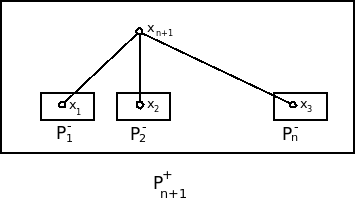
\includegraphics[scale=0.5]{figures/Figure1.png}
\newpage
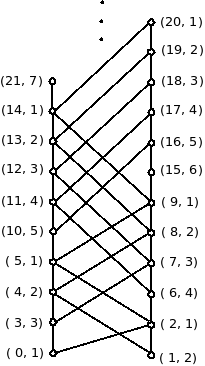
\includegraphics[scale=0.5]{figures/Figure3.png}
\newpage
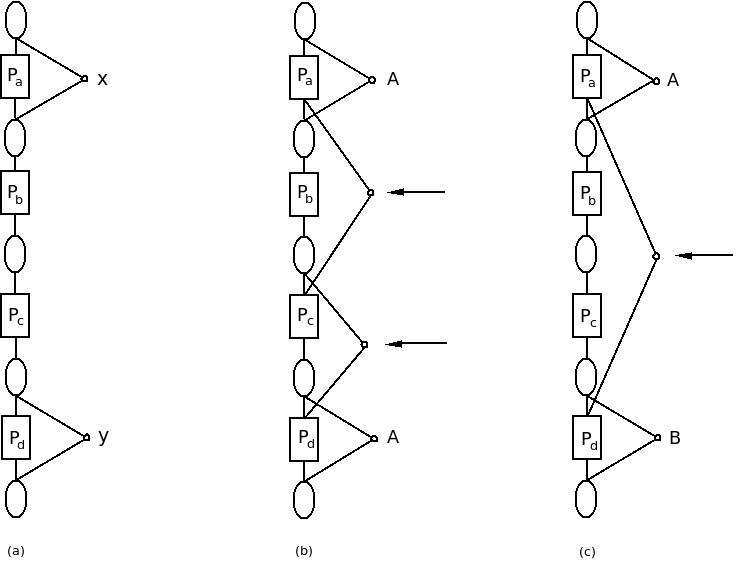
\includegraphics[scale=0.5]{figures/Figure5.png}

\end{document}
